% ****** Start of file apssamp.tex ******
%
%   This file is part of the APS files in the REVTeX 4.2 distribution.
%   Version 4.2a of REVTeX, December 2014
%
%   Copyright (c) 2014 The American Physical Society.
%
%   See the REVTeX 4 README file for restrictions and more information.
%
% TeX'ing this file requires that you have AMS-LaTeX 2.0 installed
% as well as the rest of the prerequisites for REVTeX 4.2
%
% See the REVTeX 4 README file
% It also requires running BibTeX. The commands are as follows:
%
%  1)  latex apssamp.tex
%  2)  bibtex apssamp
%  3)  latex apssamp.tex
%  4)  latex apssamp.tex
%
\documentclass[%
 reprint,
%superscriptaddress,
%groupedaddress,
%unsortedaddress,
%runinaddress,
%frontmatterverbose, 
%preprint,
%preprintnumbers,
%nofootinbib,
%nobibnotes,
%bibnotes,
 amsmath,amssymb,
 aps,
%pra,
%prb,
%rmp,
%prstab,
%prstper,
%floatfix,
]{revtex4-2}
\usepackage{braket}
\usepackage{graphicx}% Include figure files
\usepackage{dcolumn}% Align table columns on decimal point
\usepackage{bm}% bold math
\usepackage[version=4]{mhchem}
\usepackage{url}
%\usepackage{hyperref}% add hypertext capabilities
%\usepackage[mathlines]{lineno}% Enable numbering of text and display math
%\linenumbers\relax % Commence numbering lines

%\usepackage[showframe,%Uncomment any one of the following lines to test 
%%scale=0.7, marginratio={1:1, 2:3}, ignoreall,% default settings
%%text={7in,10in},centering,
%%margin=1.5in,
%%total={6.5in,8.75in}, top=1.2in, left=0.9in, includefoot,
%%height=10in,a5paper,hmargin={3cm,0.8in},
%]{geometry}

\begin{document}

% \preprint{APS/123-QED}

\title{State population transfers using Rabi oscillations}% Force line breaks with \\
% \thanks{A footnote to the article title}%

\author{Barak Dayan}%
 \email{barak.dayan@weizmann.ac.il}
 \author{Jeremy Raskop}%
 \email{jeremy.raskop@weizmann.ac.il}
\affiliation{%
AMOS and Department of Chemical Physics,\\
Weizmann Institute of Science, Rehovot, Israel
}%

%\noaffiliation

\author{Mahadevan Subramanian}
 \email{190260027@iitb.ac.in}
 \author{Drishti Baruah}
 \email{190260019@iitb.ac.in}
\affiliation{
 Department of Physics\\
 Indian Institute of Technology Bombay% with \\
}
%\noaffiliation

\date{\today}% It is always \today, today,
             %  but any date may be explicitly specified

\begin{abstract}
Quantum Control is a problem which has been explored in various avenues and is used extensively in physical realizations of quantum computers. Here we explore methods to complete state transfer in Rubidium 87 5S and 5P levels. Specifically the transfer we wish to build toward is the one for $\ket{F=1,m=1}$ to $\ket{F=3,m=3}$ using $\ket{F=2,m=2}$ as an intermediate state in the ladder STIRAP transfer. 
% \begin{description}
% \item[Usage]
% Secondary publications and information retrieval purposes.
% \item[Structure]
% You may use the \texttt{description} environment to structure your abstract;
% use the optional argument of the \verb+\item+ command to give the category of each item. 
% \end{description}
\end{abstract}

%\keywords{Suggested keywords}%Use showkeys class option if keyword
                              %display desired
\maketitle

\tableofcontents
%https://www.overleaf.com/project/605b64aa36e1e2425bc230ba
\section*{Introduction}
The problem of an atom interacting with an electromagnetic had received semi-classical treatments which had however failed to explain all the characteristics of such a system. It received a proper quantum treatment where the field was quantized in the Jaynes-Cummings Hamiltonian \cite{jaynes-cumming}. This succesfully explained very important characteristics of the system like Rabi oscillations \cite{PhysRev.51.652} and the collapse and revival of the system \cite{PhysRevLett.44.1323,Collapse}. Currently Rabi oscillations are extensively used for quantum information processing \cite{10.5555/1972505}\\
In section I we explore the nature of these Rabi oscillations and their signature behavior. In section II we explore the theory behind driving Rabi oscillations in Rubidium-87 and reach two constants which are proportionality constants for the Rabi oscillations we wish to drive given by $\mathcal{K}_{1,2}$ and $\mathcal{K}_{2,3}$. In section III, along with some STIRAP theory we present simulations for state population transfer from $\ket{F=1,m=1}$ to $\ket{F=3,m=3}$ using $\ket{F=2,m=2}$ as an intermediate state in the ladder STIRAP.

\section{Rabi Oscillations}
\subsection{Jaynes-Cummings Hamiltonian}
A two-state atom, with two energy eigenvalues, is described by a state space spanned by the two energy eigenstates $\ket{e}$ and $\ket{g}$. An arbitrary state vector $\ket{\psi(t)}$ can be expressed as a superposition of the two orthogonal states:
\begin{equation}
    \ket{\psi(t)}= c_g\ket{g}+c_e\ket{e}
\end{equation}
The Hamiltonian operator of the two-level atom in the energy representation is
\begin{equation}
    \textbf{H}_A=E_e\ket{e}\bra{e}+E_g\ket{g}\bra{g}
\end{equation}
Setting the zero of energy to the ground state energy of the atom simplifies this to ${\displaystyle {\textbf{H}}_A=E_{e}|e\rangle \langle e|=\hbar \omega _{eg}|e\rangle \langle e|}$ where ${\displaystyle \omega _{eg}}$ is the resonance frequency of transitions between the sub-levels of the atom.
\begin{equation}
    {\displaystyle {\textbf{H}}_{F}=\hbar \omega _{c}{\Bigg (}{\hat {a}}_{c}^{\dagger }{\hat {a}}_{c}+{\frac {1}{2}}{\Bigg )}}
\end{equation}
$\textbf{H}_{F}$ is the Hamiltonian of the quantized electromagnetic field where we are only considering the resonant mode of the cavity.\\
Now we obtain the dipole atom-field interaction Hamiltonian, given by, $\textbf{H}_{A-F}=-\overrightarrow{\textbf{d}}\cdot\overrightarrow{E}(\overrightarrow{x_A},t)$.\\
The dipole moment operator is represented by
\begin{equation}
    \overrightarrow{\textbf{d}}=-(\boldsymbol{\sigma^-}\overrightarrow{M}^\star-\boldsymbol{\sigma^+}\overrightarrow{M})
\end{equation}
where the dipole matrix element $\overrightarrow{M}=\epsilon_0\braket{g|\overrightarrow{x}|e}$.
We assume that the electric field is due to a monochromatic electromagnetic wave (as per the Jaynes Cummings model). So the electric field of the single mode is given by  ${\displaystyle {\hat {\vec {E}}}={\sqrt {\frac {2\pi \hbar \omega _{c}}{V}}}{\vec {u}}_{c }\left({\hat {a}}_{c }-{\hat {a}}_{c }^{\dagger }\right)}$. We define ${\displaystyle \hbar g_{c }=i{\sqrt {\frac {2\pi \hbar \omega _{c}}{V}}}\langle e|{\hat {\vec {d}}}|g\rangle \cdot {\vec {u}}_{c }}$. Thus we get
\begin{equation}
    {\displaystyle {\textbf{H}}_{AF}=\hbar {\big [}(g_{c}{\hat {\sigma }}_{+}{\hat {a}}_{c}-g_{c}^{*}{\hat {\sigma }}_{-}{\hat {a}}_{c}^{\dagger })+(g_{c}^{*}{\hat {\sigma }}_{-}{\hat {a}}_{c}-g_{c}{\hat {\sigma }}_{+}{\hat {a}}_{c}^{\dagger }){\big ]}}
\end{equation}
where ${\displaystyle {\hat {\sigma }}_{+}=|e\rangle \langle g|}$, ${\displaystyle {\hat {\sigma }}_{+}=|e\rangle \langle g|}$ and ${\displaystyle {\hat {\sigma }}_{-}=|g\rangle \langle e|}$, ${\displaystyle {\hat {\sigma }}_{-}=|g\rangle \langle e|}$ are the raising and lowering operators.\\
We go into the Hamiltonian picture to study the time dependence and get:  (${\displaystyle {\textbf {H}}_{0}={\textbf {H}}_{A}+{\textbf{H}}_{F}}$)
\begin{align}
\displaystyle {\textbf{H}}_{AF}(t)&=e^{i{\hat {H}}_{0}t/\hbar }{\textbf {H}}_{AF}e^{-i{\hat {H}}_{0}t/\hbar }\nonumber\\&=\hbar {\big (}g_{c}{\hat {\sigma }}_{+}{\hat {a}}_{c}^{\dagger }e^{i(\omega _{c}+\omega _{eg})t}+g_{c}^{*}{\hat {\sigma }}_{-}{\hat {a}}_{c}e^{-i(\omega _{c}+\omega _{eg})t}\nonumber\\&-g_{c}^{*}{\hat {\sigma }}_{-}{\hat {a}}_{c}^{\dagger }e^{-i(\omega _{eg}-\omega _{c})t}-g_{c}{\hat {\sigma }}_{+}{\hat {a}}_{c}e^{i(\omega _{eg}-\omega _{c})t}{\big )}
\end{align}
Now we make the \textbf{Rotating Wave approximation} ${\displaystyle |\omega _{eg}-\omega _{c}|\ll \omega _{eg}+\omega _{c}}$ which holds due to resonance and we can ignore the anti-resonant terms altogether. So we get
\begin{equation}
    \textbf{H}_{AF}(t)=-\hbar {\big (}g_{c}^{*}{\hat {\sigma }}_{-}{\hat {a}}_{c}^{\dagger }e^{-i(\omega _{eg}-\omega _{c})t}+g_{c}{\hat {\sigma }}_{+}{\hat {a}}_{c}e^{i(\omega _{eg}-\omega _{c})t}{\big )}
\end{equation}
$\delta=\omega_{eg}-\omega_c$ is called the detuning between field and atomic resonance.\\
We finally go back to the Schrodinger's picture and get
\begin{align}
    {\textbf {H}}_{AF} &= e^{-i{\hat {H}}_{0}t/\hbar}{\textbf {H}}_{AF}(t)e^{i{\hat {H}}_{0}t/\hbar}\nonumber\\
    &= \hbar g_{c}{\big (}{\hat {\sigma}}_{+}{\hat {a}}_{c}+{\hat {\sigma }}_{-}{\hat {a}}_{c}^{\dagger }{\big )}
\end{align}
So the full Jaynes-Cummings Hamiltonian is given as follows: (ignoring the constant term $1/2\hbar\omega_c$, which represents the zero-point energy)
\begin{gather}
    \textbf{H}_{JC} =\textbf{H}_{A}+\textbf{H}_{F}+\textbf{H}_{A-F}\nonumber\\
    =\hbar\omega_c\hat{a_c}^\dagger\hat{a_c}+\hbar\omega_{eg}|{e}\rangle\langle{e}|+\hbar g_c(\hat{\sigma_+}\hat{a_c}+\hat{\sigma_-}\hat{a_c}^\dagger)
\end{gather}
\subsection{The Maxwell-Bloch equations}
We can describe our two-level system using a density matrix 
\begin{equation*}
\rho =
\begin{bmatrix}
\rho_{ee} & \rho_{eg}\\ 
\rho_{ge} & \rho_{gg}
\end{bmatrix}
\end{equation*}
Then the time evolution of the components of this matrix is described using the following equations: (Here $\delta$ is the detuning, $\gamma$ is the decay constant of the atom, $\kappa$ is the cavity dissipation rate, ${\displaystyle {\bar {\rho }}_{ge}\equiv \rho _{ge}e^{-i\delta t}}$ and ${\displaystyle {\bar {\rho }}_{eg}\equiv \rho _{eg}e^{i\delta t}}$).
\begin{gather}
    {\frac  {d\rho _{{gg}}}{dt}}=\gamma \rho _{{ee}}+{\frac  {i}{2}}(\Omega ^{*}{\bar  \rho }_{{eg}}-\Omega {\bar  \rho }_{{ge}})\\
    {\frac  {d\rho _{{ee}}}{dt}}=-\gamma \rho _{{ee}}+{\frac  {i}{2}}(\Omega {\bar  \rho }_{{ge}}-\Omega ^{*}{\bar  \rho }_{{eg}})\\
    {\frac  {d{\bar  \rho }_{{ge}}}{dt}}=-\left({\frac  {\gamma }{2}}+i\delta \right){\bar  \rho }_{{ge}}+{\frac  {i}{2}}\Omega ^{*}(\rho _{{ee}}-\rho _{{gg}})\\
    \frac{d \bar \rho_{eg}}{dt} = - \left( \frac{\gamma}{2} - i\delta \right) \bar \rho_{eg} + \frac{i}{2}\Omega(\rho_{gg} - \rho_{ee})
\end{gather}
Upon analysing the population of the two atomic states as a function of time, we observe an oscillation in the population difference. This oscillation is called the \textbf{Rabi-oscillation}. It occurs with a frequency called the Rabi frequency, defined as ${\displaystyle \Omega ={\vec {d_{g,e}}}\cdot {\vec {E_{0}}}/\hbar }$.
\begin{figure}[ht]
    \centering
    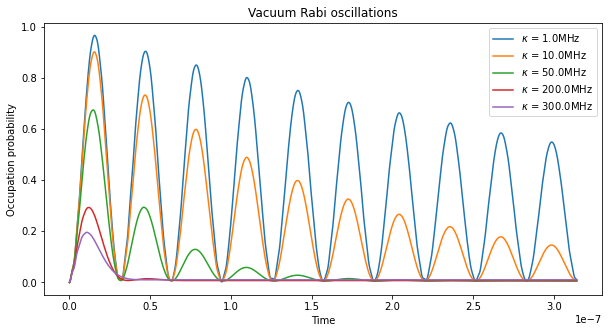
\includegraphics[width=0.5\textwidth]{images/vacuum rabi.png}
    \caption{Shown above is a simulation of a two level atom which has been entangled with a cavity with 16 fock states which starts off in the first excited state. QuTip \cite{Johansson_2012,Johansson_2013} has been used for the simulation. The value of the coupling $g = 100$ MHz, the decay for the atom is $\gamma = 3$ MHz and the cavity decay is $\kappa$ which is varying.}
\end{figure}
\begin{figure}[ht]
    \centering
    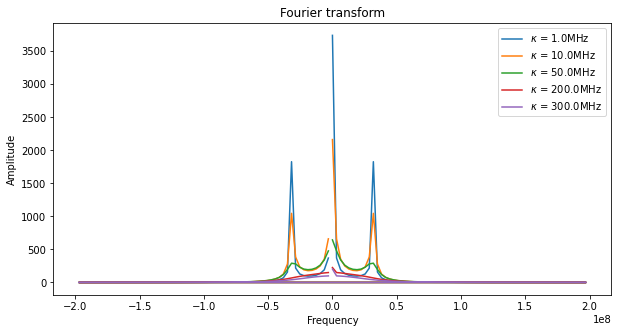
\includegraphics[width=0.5\textwidth]{images/vacuum rabi modes.png}
    \caption{Fourier transform of the Rabi oscillations shown in the previous figure. As we can see, we have three modes arise as shown in \cite{jaynes-cumming}.}
\end{figure}
\subsection{Collapse and revival of Atomic Oscillations}
The interaction Hamiltonian can only cause transitions
of the type $\ket{e}\ket{n}\leftrightarrow\ket{g}\ket{n+1}$, where these product states are refered to be as the bare states of the Jaynes-
Cummings model. For a fixed $n$, the dynamics of the system are confined to the two dimensional space of product
states $\{\ket{e}\ket{n},\ket{g}\ket{n+1}\}$.

The Jaynes-Cummings Hamiltonian can be written as:
\begin{equation}
\hat{H}_{JC}=
 \begin{bmatrix}
 n\hbar\omega_c+1/2\hbar \omega_0 & \hbar\Omega\sqrt{n+1} \\
 \hbar\Omega\sqrt{n+1} &  (n+1)\hbar\omega_c-1/2\hbar \omega_0
 \end{bmatrix}   
\end{equation}
where the eigenvalues are 
\begin{equation}
    E_\pm = (n+\frac{1}{2})\hbar\omega_0 \pm \hbar\sqrt{(\omega_0-\omega_k)^2+4\Omega^2(n+1)}
\end{equation}
On resonance, we get 
\begin{equation}
    E_\pm = (n+\frac{1}{2})\hbar\omega_0 \pm g_0\hbar\sqrt{(n+1)}
\end{equation}
where $g_0=2\Omega$.
Upon further calculations\cite{Collapse}, we find that the expression for the population inversion of atomic levels is given by 
We realise upon plotting this that collapse and revival occurs in case of interaction of a two-level atom with a cavity prepared
in a coherent way.
\begin{equation}
    W(t)=e^{-N}\sum\limits_{n=0}^\infty\frac{N^n}{\sqrt{n!}}\cos{2\Omega_r\sqrt{n+1}t}
\end{equation}
It has been shown \cite{PhysRevLett.44.1323} that the Rabi
oscillations decay at an early stage of the atom–field
interaction and reappear at a later stage, but with a
smaller amplitude. The following plot shows the occurrence of collapse and revival upon plotting the occupation probability of population in the excited state with respect to time.
\begin{figure}[ht]
    \centering
    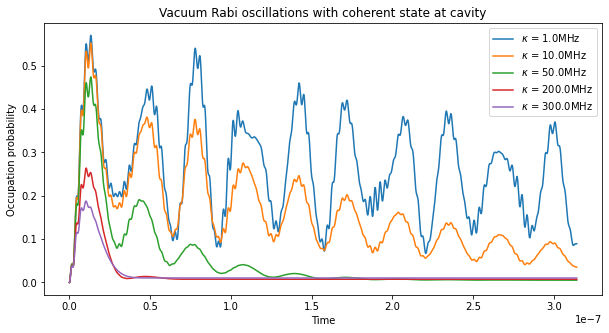
\includegraphics[width=0.5\textwidth]{images/coherent rabi.png}
    \caption{Shown above is a simulation of a two level atom which has been entangled with a cavity with 16 fock states which starts off in the coherent state with $\alpha=1$. The value of the coupling $g = 100$ MHz, the decay for the atom is $\gamma = 3$ MHz and the cavity decay is $\kappa$ which is varying.}
\end{figure}
\begin{figure}[ht]
    \centering
    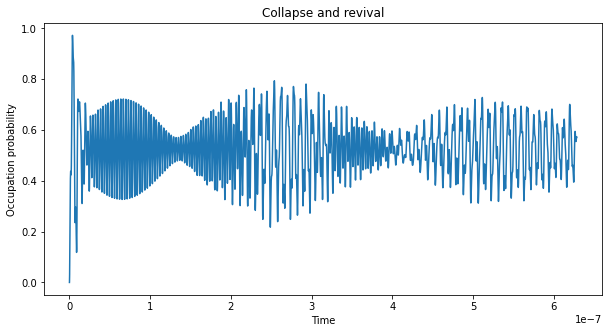
\includegraphics[width=0.5\textwidth]{images/collapse and revival 3}
    \caption{Demonstration of collapse and revival for a cavity with 32 fock states which starts off in the coherent state of $\alpha=4$. As we can see the probability dies down and goes to 0.5 a little after 0.1$\mu$s and then again rises and oscillates.}
\end{figure}

\section{Rabi Oscillations in Rubidium-87}
Rubidium-87 is one of the two naturally occiring isotopes of Rubidium other than \ce{^{85}Rb}. Due to it's energy level structure and certain characteristics, it is quite a popular atom for quantum and atom optics experiments. We will first discuss the hyperfine structure of \ce{^{87}Rb}.

\subsection{Hyperfine structure of \ce{^{87}Rb}}
\begin{figure}[ht]
    \centering
    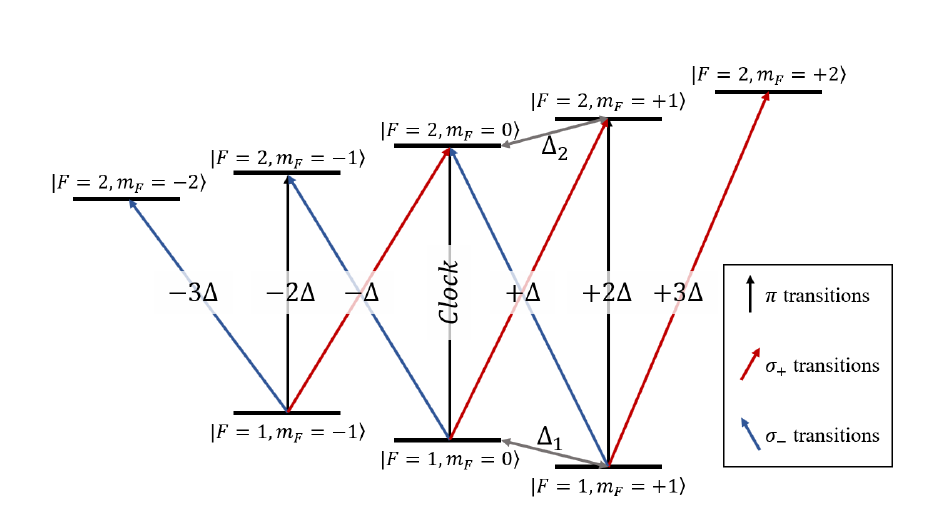
\includegraphics[width=0.5\textwidth]{images/hyperfine.png}
    \caption{Hyperfine splitting of levels in Rubidium-87. Image taken from \cite{microwavejoslin}}
    \label{fig:1}
\end{figure}
The ground state of \ce{^{87}Rb} which is the $5^2$S$_{1/2}$ undergoes a splitting as can be seen figure \ref{fig:1}. The notation for the state follows as $n^{2S+1}$L$_{J}$. There are two hyperfine levels formed due to the coupling between the total electron angular momentum ($\textbf{J} = \textbf{L} + \textbf{S}$) and the nuclear angular momentum ($\textbf{I}$) and so we write the total angular momentum as $\textbf{F} = \textbf{J} + \textbf{I}$. Here $\textbf{L}$ and $\textbf{S}$ are the orbital angular momentum and for the electronic ground state we would have $J = 1/2$ since $L=0$, $S = 1/2$ and nuclear spin is $I = 3/2$ \cite{pubchem-rb87}, Now for the addition of angular momentum we have $F$ range between $|J-I|$ and $J + I$ in integer steps. Hence for the state with $L = 0$ we only can have $F = 1,2$ with each hyperfine level split into $2F+1$ magnetic sub-levels.\\
Using the dipole moment spherical tensor as that for defining state transfer we can see using the Wigner-Eckhart Theorem \cite{book:17486} that we would require $\Delta F = 0,\pm1$ and $\Delta m_F$. The $\Delta F=0$ transitions occur in radio frequency ($10^4-10^5$ Hz) and $\Delta F = \pm1$ are in the microwave region and is about 6.8 GHz \cite{microwavejoslin}. The hyperfine Hamiltonian which describes the coupling between $\textbf{J}$ and $\textbf{I}$ has the following form \cite{rb87dline}.
\begin{eqnarray}
    \label{eq:1}H_{hfs} = \left(A_{hfs} + \dfrac{3B_{hfs}}{4I(2I-1)J(2J-1)}\right)\textbf{I}\cdot\textbf{J}
    \nonumber\\+ B_{hfs}\dfrac{3(\textbf{I}\cdot\textbf{J})^2 - I(I+1)J(J+1)}{2I(2I-1)J(2J-1)}
    %\Delta E_{hfs} = \dfrac{1}{2}A_{hfs}K + \nonumber\\ B_{hfs}\dfrac{1.5K(K+1) - 2I(I+1)J(J+1)}{2I(2I-1)2J(2J-1)}
\end{eqnarray}
We define $K = F(F+1) - I(I+1) - J(J+1)$. The $L=0\to L=1$ transition is referred to as the D line and due to the coupling is split into two components, the D$_1$ line ($5^2$S$_{1/2}\to5^2$P$_{1/2}$) and the D$_2$ line ($5^2$S$_{1/2}\to5^2$P$_{3/2}$) and equation \ref{eq:1} shows the hyperfine Hamiltonian for both these transitions.\\
Here $A_{hfs}$ is the magnetic dipole constant and $B_{hfs}$ is the electric quadrupole constant. We can see that the $B_{hfs}$ term is only of concern for the D$_2$ transition when $J\neq 1/2$ and so for now is not of any concern to us since we are interested in the microwave transition.\\
The value $A_{hfs} = \hbar 3.41734130545215(5)$ GHz is also referred to as the hyperfine structure constant \cite{hyperfineconst}. The eigen energies for $H_{hfs}$ can be seen to be $A_{hfs}K/2$ and corresponds to $-1.25A_{hfs}$ and $0.75A_{hfs}$ for $F=1$ and $F=2$ respectively. The total splitting hence is $2A_{hfs} = \hbar 6.8346826109043(1)$ GHz.

\subsection{Rabi Oscillations for the hyperfine splitting}
In the presence of a static magnetic field the Hamiltonian of the atom is the following
\begin{equation}
    H_B = \mu_B\textbf{B}\cdot(g_S\textbf{S} + g_I\textbf{I})
\end{equation}
Here the $g_S = 2.0023193043737(80)$ and $g_I = -0.0009951414(10)$ which are the Land\'e $g$ factors for electronic spin and nucleus respectively. We have the magnetic moments defined as $\vec{\mu}_L = -\mu_Bg_L\vec{L}$, $\vec{\mu}_S = -\mu_Bg_S\vec{S}$ and . From the addition of angular momenta which is $\textbf{J} = \textbf{L} + \textbf{S}$ we have the following expression for $g_J$ \cite{book17125}
\begin{eqnarray}
    g_J = g_L\dfrac{J(J+1) - S(S+1) + L(L+1)}{2J(J+1)}\nonumber\\
    +g_S\dfrac{J(J+1) + S(S+1) - L(L+1)}{2J(J+1)}
\end{eqnarray}
For the addition of $\textbf{F} = \textbf{J} + \textbf{I}$ we similarly can write the expression as
\begin{eqnarray}
    g_F = g_L\dfrac{F(F+1) - S(S+1) + L(L+1)}{2F(F+1)}\nonumber\\
    +g_S\dfrac{F(F+1) + S(S+1) - L(L+1)}{2F(F+1)}
\end{eqnarray}
In the low field limit we have the Zeeman splitting caused by magnetic field to be much smaller than the hyperfine splitting and so can be written in the following linear form of $H_B = \mu_Bg_F\textbf{F}\cdot\textbf{B}$. As shown in figure \ref{fig:1}, we can see that the splitting constant for a bias field along $z$ axis would be $\Delta = \mu_Bg_Fm_F \approx 700$ Hz/mG \cite{microwavejoslin}. At higher fields one would have to use the Breit-Rabi formula which has it's second order shown in \cite{rb87dline} but will not be of our concern here.\\
Similar to static fields, oscillating microwave fields (which will be of our main interest here) interact via the following Hamiltonian
\begin{equation}
    H_B = \mu_Bg_S\textbf{B}\cdot\textbf{S}
\end{equation}
Note that we have ignored the contribution from the nuclear angular momentum since $g_I$ is very small in comparison to $g_S$. We will be using an oscillatory magnetic field to create Rabi oscillations between the hyperfine levels.
For an example we can pick the $\pi$ transitions which will be referred to as clock transitions. Using RWA the matrix form of the hamiltonian for clock transition levels is written as follow
\begin{equation}
    H_0 = \hbar\omega_0\begin{pmatrix}\frac{3}{8}&0\\0& -\frac{5}{8}\end{pmatrix}
\end{equation}
In the interaction picture the hamiltonian in presence of a magnetic field will be written as follows (here $\Sigma_i = I_{n uc}\otimes\sigma_i$)
\begin{equation}
    H_{B,I} = e^{\iota H_0t/\hbar}\left(\sum_{i}B_i(t)\langle F,m_F|\Sigma_i|F',m_F'\rangle\right)e^{-\iota H_0t/\hbar}
\end{equation}
The evolution of state would be given by $\iota\hbar\dot{\psi} = H_{B,I}\psi$
\begin{equation}
    \Omega_{clock} = \dfrac{\mu_Bg_sB_0}{2\hbar}
\end{equation}
To convert magnetic field to intensity we simply can use the average intensity expression for electromagnetic waves
\begin{equation}
    I = \dfrac{cB_0^2}{2\mu_0} = \dfrac{c\epsilon_0E^2_0}{2}
\end{equation}
For a more general transfer from some state $i$ to $f$ we have the following equation with the matrix element $M_{IF,\{i,f\}}$
\begin{equation}
    \Omega_{i,f} = \dfrac{\mu_Bg_sB_0}{2\hbar}M_{IF,\{i,f\}}
\end{equation}
The transition matrix here from $\ket{F,m_F}$ to $\ket{F',m_F'}$ is defined as $\bra{F,m_F}\Sigma_i\ket{F',m_F'}$. We can see that $\Sigma$ can be written as a rank 1 spherical tensor with components as $\Sigma^{(1)}_0 = \Sigma_z$, $\Sigma^{(1)}_{\pm 1} = (\mp\Sigma_x-\iota\Sigma_y)/\sqrt{2}$. The Wigner-Eckhart theorem states the following
\begin{equation}
    \bra{F,m_F}\Sigma^{(k)}_{q}\ket{F',m_F'} = \langle F||T^{(k)}||F'\rangle\langle F',1;m_F',q|F,m_F\rangle
\end{equation}
Where $\langle F',1;m_F',q|F,m_F\rangle$ is the Clebsch-Gordan coefficient \cite{book:17486}. From this we get that for the $\pi$ transition we need linearly polarized light along the $z$ axis (non zero $B_z$) and for the $\sigma_\pm$ transitions where $m_f = \pm1$ we need circularly polarized light  \cite{microwavejoslin} (RCP for $\sigma_-$ and LCP for $\sigma_+$).\\
The transition of our interest is going from $\ket{F=1,m_F=1}$ to $\ket{F=2,m_F=2}$ which is a $\sigma_+$ transition. The Zeeman effect will be null since the bias field would be set at zero and we only have an oscillatory magnetic field.
We get that the desired $\sigma_+$ transition has a matrix element that is $\sqrt{3/2}$ times that of the $\pi$ transition and grouping this along with intensity we get the following relation. 
\begin{equation}
    \Omega_{\ket{1}\to\ket{2}} = \dfrac{eg_S}{4m_e}\sqrt{\dfrac{3\mu_0I}{c}} = \mathcal{K}_{1,2}\sqrt{I}
\end{equation}
Taking $I$ to be in W/m$^2$ we get $\mathcal{K}_{1,2} \approx 9.866$ kHz$\cdot$mW$^{-0.5}$
\subsection{Rabi oscillations in the D$_2$ line}
When describing the Hamiltonian for atom-light interaction, using the RWA we get the following expression for the Rabi frequency
\begin{equation}
    \Omega = -\dfrac{\bra{g}\hat{\epsilon}\cdot \textbf{d}\ket{e}\cdot E_0}{\hbar}
\end{equation}
As shown in \cite{rb87dline}, the dipole operator has symmetries which can help us in obtaining photon scattering rates with simpler expressions. The first symmetry tells us that the decay rate $\Gamma$ is independent of the sublevel chosen for transfer which happens since the matrix elements deciding transfer from any level add up to a constant
\begin{equation}
    \sum_{q,F'}|\bra{F',m_F'+q}er_q\ket{F',m_F'}|^2 = \dfrac{2J+1}{2J'+1}|\langle J||e\textbf{r}||J'\rangle|^2
\end{equation}
If we sum the matrix elements from a single ground state sublevel t the levels in some $F'$ energy level we get the following ($A_q = |\braket{F,m_F}{F',1;(m_F-q)q}|^2$)
\begin{align}
    S_{FF'} &= \sum_{q}A_q(2F'+1)(2J+1)\begin{Bmatrix}J & J' & 1\\F' & F & I\end{Bmatrix}^2\nonumber\\
    &=(2F'+1)(2J+1)\begin{Bmatrix}J & J' & 1\\F' & F & I\end{Bmatrix}^2
\end{align}
Here $\begin{Bmatrix}J & J' & 1\\F' & F & I\end{Bmatrix}$ is the Wigner-6j symbol \cite{wigner6j} which is a generalization of Clebsch-Gordan coefficients to function for addition of three angular momenta. We also note that $\sum_{F'}S_{FF'} = 1$ which shows that an isotropic pump field would couple the levels independently from their distributed populations. The factors $S_{FF'}$ decides the relative strength of the different transfers. In case the the light is isotropic and couples the two levels, the effective dipole moment is given by
\begin{equation}
    |d_{iso,eff}(F\to F')|^2 = \dfrac{S_{FF'}}{3}|\langle J||e\textbf{r}||J'\rangle|^2
\end{equation}
This gives the formula for Rabi frequency as
\begin{equation}
    \Omega_{iso} = \sqrt{\dfrac{S_{FF'}}{3}}|\langle J||e\textbf{r}||J'\rangle|\dfrac{E}{\hbar}
\end{equation}
Given that intensity is proportional to the square of peak electric field, the rabi frequency will be proportional to $\sqrt{I}$. The final expression can be written in terms of spontaneous decay rate $\Gamma$ and $I_{sat}$ which is the saturation intensity. Here $I_{sat} = \dfrac{c\epsilon_0\Gamma^2\hbar^2}{4|\hat{\epsilon}\cdot\textbf{d}|^2}$ and $\Gamma = 2\pi\cdot 6.065(9)$ MHz \cite{1996PhST...65...48V}. For the transition that we are interested in which is $\ket{F=2,m_F=2}\to\ket{F=3,m_F=3}$, we have $I_{sat} = 1.669(2)$ mW/cm$^2$ \cite{rb87dline}.
\begin{equation}
    \Omega_{\ket{2}\to\ket{3}} = \Gamma\sqrt{\dfrac{I}{2I_{sat}}} = \mathcal{K}_{2,3}\sqrt{I} 
\end{equation}
Taking $I$ to be in W/m$^2$, $\mathcal{K}_{2,3} \approx 6.590$ MHz$\cdot$mW$^{-0.5}$. Right off the bat comparing this value with $\mathcal{K}_{1,2}$, it is clear that the microwave transition requires a considerably higher amount of intensity to drive it in comparable Rabi frequencies in comparison to the optical transition.


\section{Stimulated Raman Adiabatic Passage}
\begin{figure*}[ht]
\label{fig:sim0}
    \centering
    \begin{minipage}{0.47\textwidth}
        \centering
        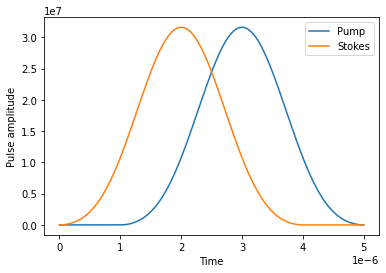
\includegraphics[width=\textwidth]{images/sim-0-pulse.png} % first figure itself
        % \caption{}
    \end{minipage}\hfill
    \begin{minipage}{0.47\textwidth}
        \centering
        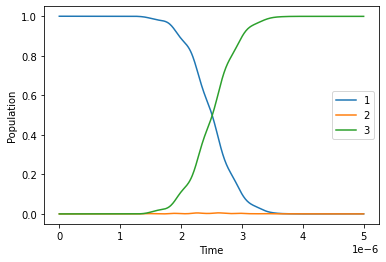
\includegraphics[width=\textwidth]{images/sim-0-pop.png} % second figure itself
        % \caption{second figure}
    \end{minipage}
    \caption{Simulation results for STIRAP using blackman shaped pulses as shown in the figure on left. Both the pulses have equal Rabi peaks of 31.6 MHz and the timescale of $T=5\mu$s and each pulse is $4\mu$s wide. The results (right) show that there is a successful transfer of about $99.95\%$ efficiency which is pretty much perfect. The $\Delta = 1$ MHz in this simulation.}
\end{figure*}
\subsection{Theory}
\begin{figure*}[ht]
\label{fig:sim1}
    \centering
    \begin{minipage}{0.47\textwidth}
        \centering
        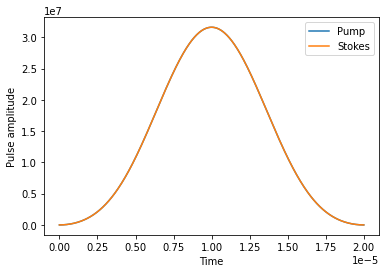
\includegraphics[width=\textwidth]{images/sim-1-pulse.png} % first figure itself
        % \caption{}
    \end{minipage}\hfill
    \begin{minipage}{0.47\textwidth}
        \centering
        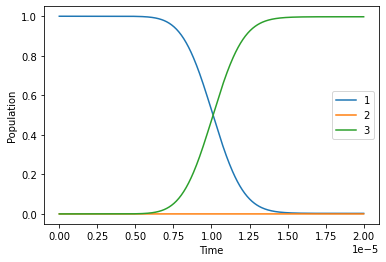
\includegraphics[width=\textwidth]{images/sim-1-pop.png} % second figure itself
        % \caption{second figure}
    \end{minipage}
    \caption{Simulation results for STIRAP using blackman shaped pulses as shown in the figure on left. Both the pulses have equal Rabi peaks of 31.6 MHz and the timescale of $T=20\mu$s and each pulse is $20\mu$s wide. The results (right) show that there is a successful transfer of about $99.5\%$ efficiency which is pretty much perfect. The $\Delta = 1$ GHz in this simulation. The interesting thing about this simulation is that the peak efficiency for this timescale was achieved when the pump and stokes laser were completely overlapping.}
\end{figure*}
\begin{figure*}[ht]
    \label{fig:sim3}
    \centering
    \begin{minipage}{0.47\textwidth}
        \centering
        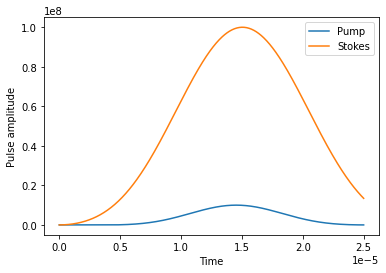
\includegraphics[width=\textwidth]{images/sim-3-pulse.png} % first figure itself
        % \caption{}
    \end{minipage}\hfill
    \begin{minipage}{0.47\textwidth}
        \centering
        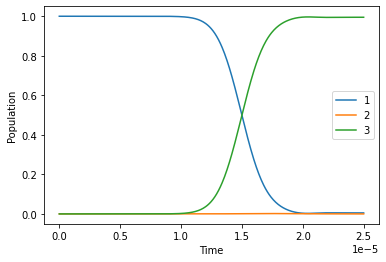
\includegraphics[width=\textwidth]{images/sim-3-pop.png} % second figure itself
        % \caption{second figure}
    \end{minipage}
    \caption{Simulation results for STIRAP using blackman shaped pulses as shown in the figure on left. The pump pulse had a peak of 10 MHz and the stokes pulse had a peak of 100 MHz and the timescale $T = 50\mu$s. Here $\Delta = 1$ GHz and $\delta = 2.182238$ MHz. The aim of this optimization was to see if the transfer can be run efficiently at a smaller timescale and using the scipy optimization we were able to run it at 25$\mu$s but not any lesser without sacrificing efficiency. The thing to take note of is that the stokes pulse actually ends at beyond the $T$ and while it may seem wrong, this is really the same as multiplying the blackman window which just got cut at the end since the simulation only runs till that point in time after which it is safe to say that both the Rabi frequencies are zero. The stokes pulse would have ended at about $1.20T$ (not considering it being set to zero at $T$) and the pump pulse begins at $0.163T$. The efficiency achieved was about 99.5\% for this parameter set and was also fairly robust to slight variations around these numbers.}
\end{figure*}
Stimulated Raman Adiabatic Passage (STIRAP) is a process which permits transfer between two states using two coherent electromagnetic pulses. The approach makes use of an intermediate state and the aim is to keep the steady state population of this intermediate state to be very small. For STIRAP \cite{73.043415} we need $\Delta_S = -\Delta_P$ for the two photon resonance in ladder configuration ($E_1<E_2<E_3$).
\begin{gather}\hbar\Delta_P = E_2 - E_1 - \hbar\omega_P\\
\hbar\Delta_P = E_3 - E_2 - \hbar\omega_S\end{gather}
The effective hamiltonian in the basis of these three states can be written as
\begin{equation}H = \dfrac{\hbar}{2}
\begin{pmatrix}0 & \Omega_P(t) & 0\\
               \Omega_P(t) & \Delta & \Omega_S(t)\\
               0 & \Omega_S(t) & \delta\end{pmatrix}
\end{equation}
We aim to transfer population from $\ket{F=1,m=1}$ to $\ket{F=3,m=3}$ using $\ket{F=2,m=2}$ as an intermediate state. Here we use $\Omega_P$ (referred to as arising from the pump laser in common text) for transfer between $\ket{F=1,m=1}$ to $\ket{F=2,m=2}$ which is microwave induced and $\Omega_S$ (referred to as arising from the stokes laser in common text) for transfer between $\ket{F=2,m=2}$ to $\ket{F=3,m=3}$ which is done by an optical laser. These have been explained in detail in the previous section.\\
We define a mixing angle $v(t)$ as $\tan(v(t)) = \Omega_P(t)/\Omega_S(t)$. When there is two photon resonance, one of the eigenvalues of the Hamiltonian is zero. The eigenstate (called as the dark state) for this eigenvalue would be
\begin{equation}
    \ket{\phi_0}
    = \cos(v(t))\ket{1} - \sin(v(t))\ket{3}
\end{equation}
As we can see, there is no population that would go to the intermediate state in such a situation and as long as the mixing angle changes slowly, we would have a successful STIRAP. Populating the second state would come with it's losses due to decay from $\ket{2}$ and so is aimed to be kept low. The other two adiabatic states are as follows \cite{doi:10.1063/1.458514}
\begin{eqnarray}
    \ket{\phi_+} = \sin(v(t))\sin(\varphi(t))\ket{1} + \cos(\varphi(t))\ket{2}\nonumber\\+\cos(v(t))\sin(\varphi(t))\ket{3}\\
    \ket{\phi_+} = \sin(v(t))\sin(\varphi(t))\ket{1} + \cos(\varphi(t))\ket{2}\nonumber\\+\cos(v(t))\sin(\varphi(t))\ket{3}
\end{eqnarray}
Here $\tan(2\varphi(t)) = \frac{\sqrt{\Omega_P(t)^2+\Omega_S(t)^2}}{\Delta}$. The eigenvalues are $\epsilon_\pm(t) = [\Delta\pm\sqrt{\Delta^2+\Omega_P(t)^2+\Omega_S(t)^2}]$. If $\Delta=0$, and at some time both the Rabi frequencies are zero, the three states are degenerate which is lifted off when any of these become non zero referred to as Autler-Townes splitting \cite{PhysRev.100.703}. The stepwise procedure for STIRAP is as follows \cite{73.043415}
\begin{itemize}
    \item \textbf{Stage 1:} $\Omega_S$ is non zero and $\Omega_P=0$ causing Autler-Townes splitting for $\ket{2}$ and $\ket{3}$. The state vector coincides with the dark state.
    \item \textbf{Stage 2:} $\Omega_S$ is much greater than $\Omega_P$ which is non zero now. The state deviates slightly from the dark state but the transfer to the two states in equations 24,25 is prevented due to the strong $S$ field causing destructive interference. 
    \item \textbf{Stage 3:} $\Omega_S$ is in same scale as $\Omega_P$ now and the mixing angle increases from 0 to $\pi/2$ and the state remains in the dark state so $\ket{2}$ is left unpopulated.
    \item \textbf{Stage 4:} The state is now nearly aligned to $-\ket{3}$ and $\Omega_P$ is much larger than $\Omega_S$ and similar to stage 2, this prevents the population in the third state to get transferred elsewhere.
    \item \textbf{Stage 5:} $\Omega_S$ is now gone and the $P$ induced Autler-Townes splitting gradually goes to zero and we have the final state as $-\ket{3}$.
\end{itemize}

Typically one would want the STIRAP to have a very low $\Delta$, $|\Omega_P|,|\Omega_S|$ should be much smaller than the energy differences and we set $\delta=0$. Under these conditions, it is seen that the results are relatively insensitive such as pulse shape and timing making the process robust \cite{stirap}. An important point to note is that under these conditions, the ordering of the pulses must be kept in mind ($SP$ order). This is also referred to as counter-intuitive pulse ordering and while the intuitive pulse ordering ($PS$) may work, it is not as robust. Additionally one can include decaying effects by writing the effective detuning as $\Delta' = \Delta - \Gamma\iota/2$ and causes an overall decay in population \cite{PhysRevA.56.1463} where $\Gamma$ is the amount of decay in Hz.\\
Taking $\ket{\psi} = a_1\ket{F=1,m=1}+a_2\ket{F=2,m=2}+a_3\ket{F=3,m=3}$, at large detunings we can take $\dot{a}_2$ to be close to zero since the oscillations of $\Delta$ would average out to zero in the timescale of the pulses \cite{book:693009},\cite{PhysRevA.55.648}. This will reduce the problem to a two dimensional one where the rabi frequency is given by
\begin{equation}\Omega_{eff}(t) = -\dfrac{\Omega_P(t)\Omega_S(t)}{\Delta}\end{equation}
\begin{equation}\Delta_{eff}(t) = \dfrac{\Omega_P(t)^2-\Omega_S(t)^2}{2\Delta}\end{equation}
To get an effective rabi frequency of 1 MHz where the detuning $\Delta = 1$ GHz we can use a microwave rabi frequency peaking at about $10$ MHz and an optical rabi frequency peaking at about $100$ MHz. \\
We know that $\Omega_S$ is proportional to $\sqrt{I}$, so for a peak intensity $I=23.02$ mW/cm$^2$, we get the peak $\Omega_S$ = 100 MHz based on the value of $\mathcal{K}_{2,3}$. Also we would have $\Omega_{\mu W}$ = 10 MHz for magnetic intensity $\approx$ 1.03 W/mm${}^2$. As we can see we have no choice but to keep unequal peaks and in the next subsection we discuss why a non zero $\delta$ is now very important for this.
\subsection{Importance of two photon detuning}
\begin{figure}[ht]
    \centering
    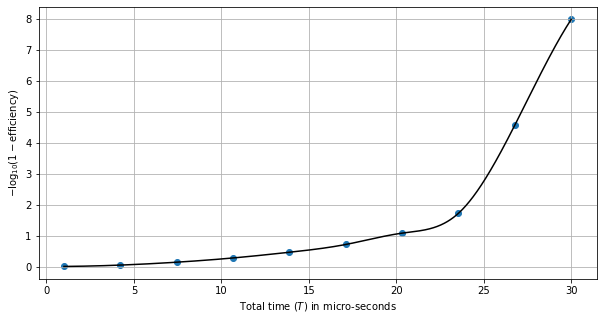
\includegraphics[width=0.47\textwidth]{images/stirap dependence on total time.png}
    \caption{For the above graph we picked 10 equally spaced points in the range of 1$\mu$s to 30$\mu$s and taking each as a value for the total time $T$ we seperately optimized their efficiency. The results show that the best possible efficiency for the STIRAP which follows our constraints clearly gets closer to 1 as the $T$ increases. The 10 data points have been connected by a cubic spline for representational purposes.}
    \label{fig:efftimes}
\end{figure}
\begin{figure}[ht]
    \centering
    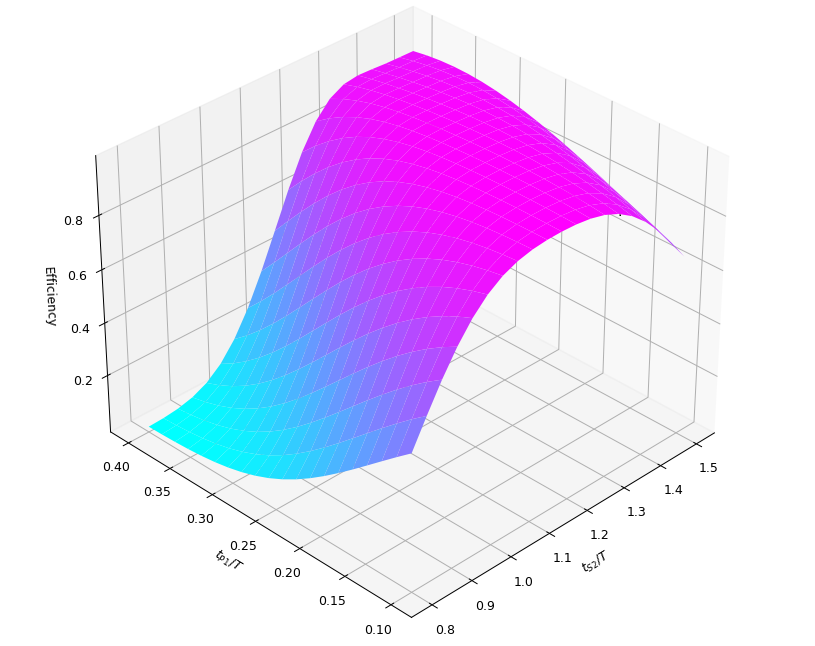
\includegraphics[width=0.5\textwidth]{images/stirap-eff-25-mu.png}
    \caption{Shown above is the variation of efficiency for the stirap based on two parameters $t_{P1}$ which is the start of pump pulse and $t_{S2}$ which is the end of the stokes pulse. The total time $T=25\mu$s here and the $\delta=2.182238$ MHz. As we can see the surface which shows the value of efficiency seems to have a well defined maximum which somewhat looks like a saddle but need not extend over the complete range to be one. We can visually see that near the maximum which was approached by our previous optimization, there are many points which still boast a very close value of efficiency showing that the choice of parameters does have some breathing space and hence demonstrating the robustness of the process.}
    \label{fig:eff25}
\end{figure}
When the Rabi
frequencies of the P and S pulses differ significantly, the optimum conditions for population transfer in an ensemble
no longer center on two-photon resonance $\delta=0$ and it may become desirable to select
a nonzero value of $\delta$ in order for the population transfer to be most effective\cite{stirap}. That is the reason we get near perfect efficiency irrespective of the value of $\delta$ upon plotting efficiency vs $\delta$ for equal Rabi
frequencies of the P and S pulses. For this, we now study how efficiency changes as we change the two-photon detuning.

\begin{figure}[ht]
    \centering
    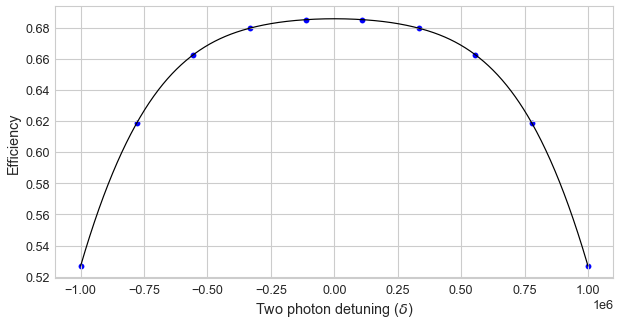
\includegraphics[width=0.47\textwidth]{images/detuning 1.png}
    \caption{In the above graph, we have plotted efficiency vs the the two photon detuning, for $T=0.5$ms,$\Omega_S=31.6$MHz,$\Omega_P=3.16$MHz,$\Delta=0,\gamma=6$MHz. Here we picked 10 equally spaced points in the range of -1$\mu$Hz to 1$\mu$Hz and plotted the efficiency, with the data points connected by a cubic spline for representational purposes.}
\end{figure}
\begin{figure}[ht]
    \centering
    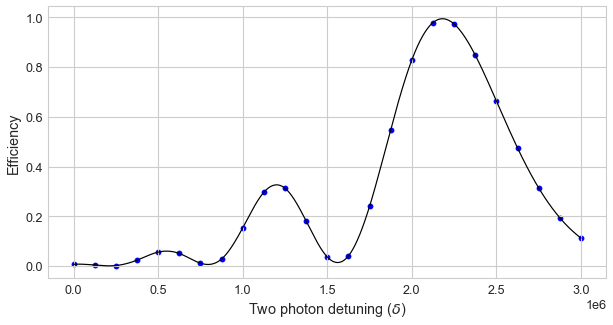
\includegraphics[width=0.47\textwidth]{images/detuning 2.png}
    \caption{In the above graph, we have plotted efficiency vs the the two photon detuning, for $T=0.25$ms,$\Omega_S=100$MHz,$\Omega_P=10$MHz,$\Delta=1$GHz,$\gamma=$0. Here we picked 25 equally spaced points in the range of 0 to 3$\mu$Hz and plotted the efficiency, with the data points connected by a cubic spline for representational purposes.}
\end{figure}

\subsection{Simulations}

% \begin{figure*}[ht]
%     \centering
%     \begin{minipage}{0.47\textwidth}
%         \centering
%         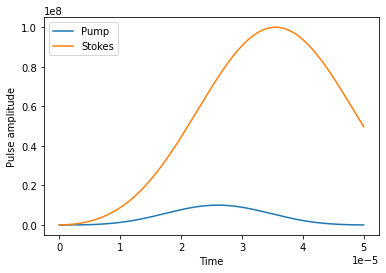
\includegraphics[width=\textwidth]{images/sim-2-pulse.png} % first figure itself
%         % \caption{}
%     \end{minipage}\hfill
%     \begin{minipage}{0.47\textwidth}
%         \centering
%         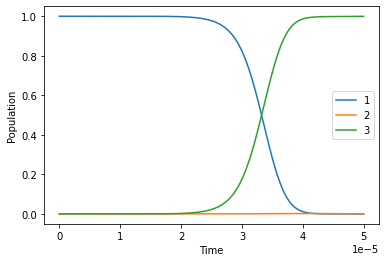
\includegraphics[width=\textwidth]{images/sim-2-pop.png} % second figure itself
%         % \caption{second figure}
%     \end{minipage}
%     \caption{Simulation results for STIRAP using blackman shaped pulses as shown in the figure on left. The pump pulse had a peak of 10 MHz and the stokes pulse had a peak of 100 MHz and the timescale $T = 50\mu$s. Here $\Delta = 1$ GHz and $\delta = 2.2529369$ MHz. The thing to take note of is that the stokes pulse actually ends at beyond the $T$ and while it may seem wrong, this is really the same as multiplying the blackman window which just got cut at the end since the simulation only runs till that point in time after which it is safe to say that both the Rabi frequencies are zero. The stokes pulse would have ended at about $1,42T$ (not considering it being set to zero at $T$) and the pump pulse begins at $0.042T$. The efficiency achieved was greater than 99.9\% for this parameter set and was also fairly robust to slight variations around these numbers.}
% \end{figure*}

QuTip \cite{Johansson_2012,Johansson_2013} was used for the simulations along with Krotov \cite{GoerzSPP2019} to both solve the equations of the time dependent Hamiltonian and change pulse shapes for optimized results. The Krotov optimization procedure used is based on an example in the documentation of the package \cite{krotov.example}. It must be noted however that the final optimization procedure used was Powell's method \cite{10.1093/comjnl/7.2.155} with help of the SciPy package. The variables which were used in the optimization were the end time of the stokes pulse, the start time of the pump pulse and the two photon detuning. The start time of stokes was trivially set to 0 and the end time of the pump was also trivially set to $T$. The final results are demonstrated in figures \ref{fig:sim0}, \ref{fig:sim1} and \ref{fig:sim3}.\\
An important requirement for a successful STIRAP transfer is that $\sqrt{\Omega_P^2+\Omega_S^2}T >> 10$ which is a limit obtained by simulations shown in \cite{RevModPhys.70.1003}. As shown in figure \ref{fig:sim3} we successfully did manage to get the simulation done for 25$\mu$s however for smaller times the optimal efficiency did not reach the desired values (see figure \ref{fig:efftimes}). We also demonstrate that the process is robust as we can see in figure \ref{fig:eff25}.
\section{Conclusion and discussion}
We have in our simulations demonstrated the successful transfer of population between $\ket{F=1,m_F=1}$ to $\ket{F=3,m_F=3}$ in the large detuning regime. A thing to note is that we have stuck to the Blackman pulse shapes throughout and while these are similar to the Gaussian (upto the sixth central moment) and very practical, one can choose more varying pulse shapes.\\
There is infact a more optimized shape presented in \cite{PhysRevA.80.013417} where Dykhne-Davis-Pechukas (DDP) method is used to minimize nonadiabatic transitions and to maximize the fidelity of the resulting STIRAP. Also when using the Krotov method to optimize pulse shapes one would often end up on a pulse which has a shape with varying phase along with varying amplitude. This however can result in significant levels of population entering the second state which combined with decay can be detrimental.\\
On an additional note we have not used the decay factor of $\Gamma$ anywhere in our simulations since even if included we would use it to be about $6$ MHz based on data discussed in previous sections and so does not actually affect our calculations much.

\section*{Acknowledgements}
We would like to thank Professor Barak Dayan for his guidance since the commencement of this project and for his support and assistance to both of us. We have learnt a lot from Professor Dayan over the course of the project and as a result have gained valuable insight into the interesting field of quantum optics. We are very grateful to have received this opportunity and to have spent our summer working on this project.

\section*{Code availability}
All the codes which were used for generating data and the plots for this report can be found at \url{https://github.com/mahadevans2432/Quantum-Optics}

% The \nocite command causes all entries in a bibliography to be printed out
% whether or not they are actually referenced in the text. This is appropriate
% for the sample file to show the different styles of references, but authors
% most likely will not want to use it.
% \nocite{*}

\bibliography{references}% Produces the bibliography via BibTeX.

\end{document}
%
% ****** End of file apssamp.tex ******
